\section{Discussion}
\label{chap1:sec:dis}

As we have shown, MMS is an effective means of diagnosing problems within 
the algorithms and implementations of isosurface extraction algorithms. 
In this work we have considered the two -- algorithm and implementation --
as one unit as one cannot always distinguish between the two if only
limited information (source code and algorithmic details) is 
available.  In this section, we present a more thorough discussion 
of the use of MMS, particularly for isosurface extraction.

\paragraph*{On the implementation and use of MMS.}
One of the primary advantages of verifying simulation codes using MMS
is that it is a non-intrusive method. MMS treats the code being
verified as a blackbox, and so can be easily integrated into an existing
test suite with little to no impact.
%
% \paragraph{On the implementation and use of MMS:} Unlike traditional
% computational simulation codes that uses MMS, Algorithm
% \ref{alg:manufactured-solutions} does not need to be integrated on the
% developing code. It treats the code under verification as a blackbox
% and therefore can be easily used with low or zero impact on any other
% test suite being used (MMS does not replace traditional test suites
% but rather complement them).
%
However, MMS does not ``see'' the implementation, and so provides
little direct information about where a particular bug might be when there
is a discrepancy between the formal and observed orders of accuracy.
In our experience, there are three main places where mistakes can happen: (1) in
the design and construction of the manufactured solution, (2) in the coding of the
algorithm being tested, and (3) in the evaluation and interpretation
of the results. Mistakes on the evaluation of results have two flavors:
misinterpretation or poor formal order of accuracy. The first heavily
depends on testers' and experts' experience and ability to judge what
a good result is. For example, should the normal observed order of accuracy for
Afront and Macet on Figure \ref{fig:normconver} be considered linear
($p = 0.80$ and $p = 0.75$ respectively)?
%
The latter depends on a rigorous formal order of accuracy analysis of the algorithm
considering all sorts of errors; even round-off errors may be
significant. In fact, we spent more time on writing out rigorously the
analysis of the formal order of accuracy and on searching for possible sources of
error than on the tests themselves. This again highlights the fact that verification 
using MMS is a process: it is typical to go back to the white board and refine
formal analyses before arriving at conclusive answers.
%
Although the formal order of accuracy analysis might be a painful
process, the literature has many results that can be promptly
used. As a consequence, if one wishes to writes his own MC technique,
for instance, his only concern is to write a test which exploits 
the results available within the literature.
% MMS itself is an
% easy-to-code test. All that is needed is to run the desired code as a
% blackbox and compute the error relative to a manufactured solution.

\paragraph*{On the complexity of the manufactured solution.}
\label{chap1:sec:mms-complexity}
The complexity of the manufactured solution can have a large influence
on the effectiveness of verification. 
Suppose one chooses the manufactured solution to be $f(x,y,z) = x + y + k
$, $k$ constant, instead of a
sphere. Since MC-based techniques use linear interpolation,
one expects the approximation
to be exact regardless of any discretization
parameter $h$, {\em i.e.}, $p = 0$ (notice that the evaluated error might
be non-zero, implying there is some other error source that
does not depend on $h$).
%
Since such a function $f$ is extremely simple,
it might not trigger bugs that would otherwise reduce the
observed order of accuracy. In our experiments, the (problematic) implementation of
Dual Contouring achieved the formal order of accuracy for this
particularly simple function ($p = 0$).
% Since this new $f$ is a really simple
% manufactured solution, Dual Contouring code (with bug) was able to
% approximate the isosurface with zero-th observed order accuracy. This
% corroborates with the correctness of the (bugged) implementation.

Another example on the influence of manufactured solution arose with
in our examination of Afront. Because Afront uses Catmull-Rom splines, some simple
isosurfaces will converge to within numerical error for very rough
volumes, and the numerically observed order of accuracy will be much
lower than expected. With an implicit function whose isosurfaces are
spheres, we observed zero-th order of accuracy for Afront for algebraic distance. 
With a modified implicit function that included transcendental functions, 
MMS reveals that Afront does not have the expected convergence rate on the 
full interval, as shown in
Figure~\ref{fig:afront-meshconvonh}. Notice that Macet has similar behavior.
Additional tests are needed to determine the source 
of this behavior within both codes.

% %  concerns Afront code. A possible input data for Afront is
% % a voxelized grid, the same grid used by MC-based techniques. The first
% % step for Afront is to build a implicit surface using Catmull-Rom
% % splines locally so that the guidance field might be constructed
% % later. Furthermore, every mesh vertex is projected onto the spline
% % (i. e., the error on mesh vertices depends on the quality of spline
% % approximation). In the tests perfomed in Section
% % \ref{chap1:sec:verification-results}, we were refining $\rho$ and
% % maintaining the voxel size $h$ fixed, so that we could evaluate
% % convergence on $\rho$. This test indirectly evaluates the correctness
% % of Catmull-Rom splines construction, although this is not the best way
% % to evaluate it. Thus, since Afront uses Catmull-Rom splines for
% % function approximation one might expect cube order of accuracy for
% % Afront on mesh vertices.
% % Nevertheless, the observed order on $h$ for Afront using a sphere as a
% % manufactured solution is $p = 0$. This is due to Catmull-Rom spline
% % ability to approximate a sphere with high precision and then the
% % approximation error is constant, $E_{k} = \max_{j=1\cdots n}|v -
% % f(c_{\sigma_j})| \approx 10^{-5}$, regardless of $h$ (note that this
% % error is less than any other error found previously for centroid
% % convergence). 

% Using a more complex manufactured solution, namely,
% $f(x,y,z) = a \cos(x) \cos(y) - z_0$, where $a$ is amplitude and $z_0$
% fixed, we observe a \emph{linear} convergence rate (Figure
% \ref{fig:afront-meshconvonh}). This might be due to a bad test, a poor
% convergence analysis or a bug in the code.

\begin{figure}
\centering
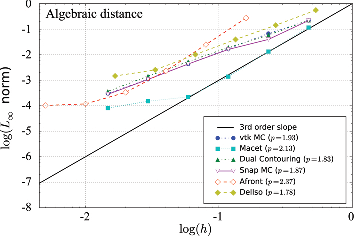
\includegraphics[width=0.84\linewidth,keepaspectratio=true]{chapter2/figures/afront_meshconv-onh.pdf}
  \caption{Order of accuracy for a transcendental function 
$f(x,y,z) = x^2 + y^2 + z^2 + \cos(Ax)^2 + \cos(Ay)^2 + \cos(Az)^2$, $A$ 
is a constant. The observed orders of accuracy for all implementations 
are relative to the voxel size $h$.
We expect third-order accuracy for 
Afront and Macet due to their use of high-order spline approximations.
Both have the expected convergence rate for all but the last two values.}
  \label{fig:afront-meshconvonh}
\end{figure}

\paragraph*{On the order of accuracy.}
In this paper, we have chosen to make our formal analysis as generic
as possible to accommodate as many implementations under verification
as possible. Although we are able to evaluate many codes using the same 
manufactured solution, when using MMS for a particular code, it is best to
exploit as much detail about the algorithm as necessary. If the goal is to 
design a manufactured solution for verifying Marching Cubes-based techniques 
the manufactured solution should exercise all possible cases. % Both functions presented
% before touches at most 102 table entries ($\sim 40\%$ of the MC table)
% and thus they are imcomplete tests.
Additionally, particular aspects of the manufactured solutions can be
incorporated into the formal analysis. For example, the analysis for
Afront becomes much more complicated if curvatures are not constant
over the surface (in that case, its additional parameter $\eta$ comes
into play~\cite{Schreiner06}, and accurately bounding the triangle
size is not practical).

%When evaluating the errors generated by the approximations, there are
%two main issues. First, one needs to decide where to evaluate the
%error. 

The errors in Section~\ref{chap1:sec:verification-results} were
measured at different locations on the mesh. Vertex convergence and
Gaussian curvature were measured on triangle vertices, while normals
were measured on the triangle centroid. 
More importantly, measurements
performed at different locations may have different orders of
accuracy. For example,
Macet has cubic formal order of accuracy on vertices due to the spline approximation
but quadratic formal order of accuracy on centroids.

In Section~\ref{chap1:sec:iea}, we define the error using a pessimistic
$L_\infty$ norm. This makes MMS a very sensitive technique. In
fact, it can detect subtle off-by-one mistakes in grid sizes
and interactions between node-centric and cell-centric
reconstructions,
even for simple manufactured solutions. In
these cases, it is important not to infer incorrect conclusions. 

% Carlos: I removed this - it does not seem important.
%
% Consider advancing front techniques. Besides
% the challenge of placing a triangle on the mesh, algorithms based on
% advancing front technique have to deal with fronts that meet. At this
% point, the algorithm might be forced to insert a ``bad triangle'',
% which might cause a drastic change in $L_\infty$ norm. Therefore, if
% we define a loose norm $|| \ast ||_\star = \frac{1}{d} || \ast ||_1$,
% which is the average error on a $d$-dimensional vector, the observed
% order of accuracy for Afront and VTK Marching Cubes becames $p = 0.94$
% and $p = 0.99$ respectively. Both results are close to the ideal
% linear order. The formal analysis for $L_\infty$ is usually simpler,
% but the particular choice will depend on context.

The numerical estimates for MMS should be performed on as wide a range
of parameter values as possible. In our tests, we used 
$h \in (0.001, 1.0)$ and observed that both faulty implementations
performed appropriately for large values of $h$. Just as the
implementations might only enter the asymptotic regime and achieve the
formal convergences for small values of $h$, it might be that (as we
have experienced) bugs only manifest themselves on sufficiently small
values of $h$.

% Besides of the range of values, we may identify more code mistakes if
% we perform evaluation for as many different functions as possible
% (area, normal, curvature, etc). For instance, although the observed
% order for Macet on interval $h \in [4^{-2}, 4^{0}]$ is acceptable for
% algebraic distance and area, it is not satisfactory for normal and
% this might be enough to revisit the code and motivates new tests.

% Finally, all functions defined over the surface have a well defined
% observed order of accuracy except for gaussian curvature, which is
% $O(1)$. The constant formal order of accuracy $O(1)$ does not allow us
% to draw any conclusion about the correctness of the code.

% If we intend to use the method outside this interval we should apply the method for that interval.

\paragraph*{On the limitations of the test.}
MMS does not cover every aspect of verification for
isosurface extraction. For example, an important aspect we do not
know how to test with MMS is the topological correctness of an
extracted mesh. This is challenging because there does not seem to
be a good measure of convergence for topological properties
such as the Euler characteristic or Betti numbers. A proper study of
these issues is a natural avenue for future work.

%
%
% In a extreme case, we could have a
% isosurface extractor algorithm that converges for every MMS solution
% but fails to generate a mesh with same topology of the input
% surface. This fails because our convergence tests does not consider
% more than a neighborhood of a point to compute the desired properties.

